\section{Test results}

After performing the described tests we ended up with quite a lot of data. The various test results are summarized in figures, some of which are included further on in this chapter to illustrate interesting and valuable observations.

\subsection{Agreements}

Looking at the Average test agreements in Figure \ref{fig:18_agreements} and \ref{fig:180_agreements}, we see that with a tighter deadline, we achieve less agreements compared to the scenario with a 180-round cap.

\begin{figure}[H]
	\minipage{0.49\textwidth}
	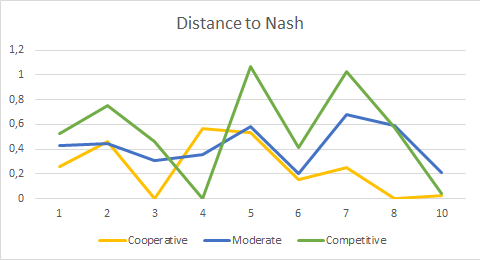
\includegraphics[width=\linewidth]{pre/18_distance_nash}
	\caption{18 Rounds per Opponent}
	\label{fig:18_distance_nash}
	\endminipage\hfill
	\minipage{0.49\textwidth}
	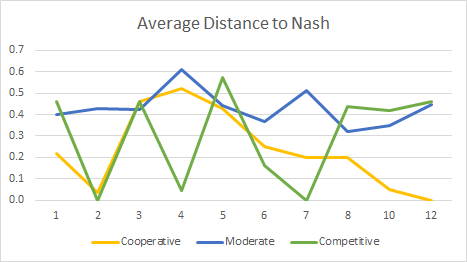
\includegraphics[width=\linewidth]{pre/180_distance_nash}
	\caption{180 Rounds per Opponent}
	\label{fig:180_distance_nash}
	\endminipage\hfill
\end{figure}

\subsection{Distances to Nash and Pareto}

Figures \ref{fig:18_distance_nash} and \ref{fig:180_distance_nash} show the average distance to Nash for each set of tournaments. We see that on the longer negotiations, bids with a lower distance to Nash are found and used. This results in lower distances to Nash. The same can be observed from the average distance to Pareto in Figure \ref{fig:18_distance_pareto} and \ref{fig:180_distance_pareto}.

\begin{figure}[H]
	\minipage{0.49\textwidth}
	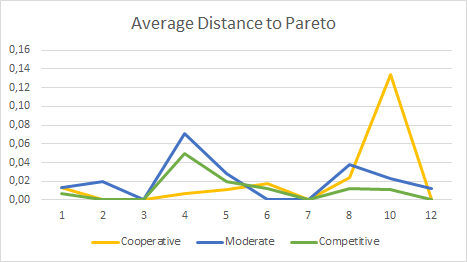
\includegraphics[width=\linewidth]{pre/18_distance_pareto}
	\caption{18 Rounds per Opponent}
	\label{fig:18_distance_pareto}
	\endminipage\hfill
	\minipage{0.49\textwidth}
	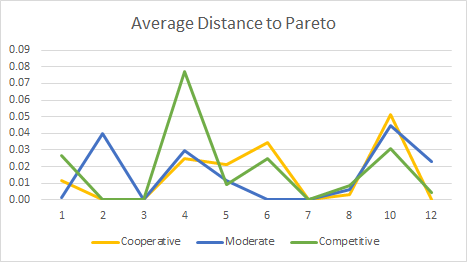
\includegraphics[width=\linewidth]{pre/180_distance_pareto}
	\caption{180 Rounds per Opponent}
	\label{fig:180_distance_pareto}
	\endminipage\hfill
\end{figure}

\subsection{Number of Rounds}

The number of rounds it takes to reach an agreement (Figure \ref{fig:18_rounds} and \ref{fig:180_rounds}) is relatively the same for both 18- and 180-capped sessions. It can also be observed that the opponents that we reach a lower amount of agreements with, generally take more rounds to that agreement.\\

\begin{figure}[H]
	\minipage{0.49\textwidth}
	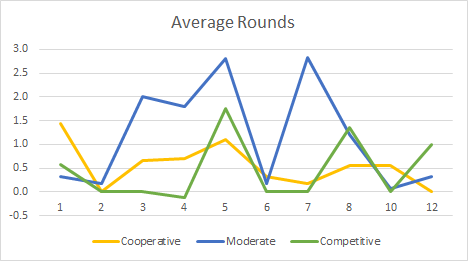
\includegraphics[width=\linewidth]{pre/18_rounds}
	\caption{18 Rounds per Opponent}
	\label{fig:18_rounds}
	\endminipage\hfill
	\minipage{0.49\textwidth}
	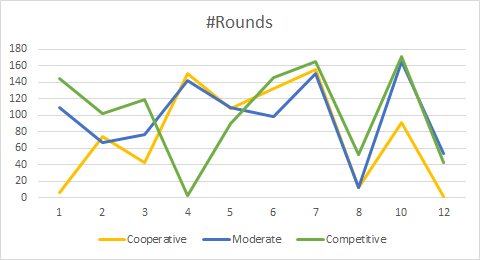
\includegraphics[width=\linewidth]{pre/180_rounds}
	\caption{180 Rounds per Opponent}
	\label{fig:180_rounds}
	\endminipage\hfill
\end{figure}

\subsection{Social Welfare}

Despite the bigger distances to Nash and Pareto, Figure \ref{fig:18_social_welfare} and \ref{fig:180_social_welfare} show that the average Social Welfare for both short and long negotiations are practically identical. \\

\begin{figure}[H]
	\minipage{0.49\textwidth}
	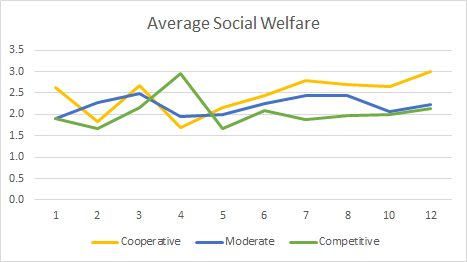
\includegraphics[width=\linewidth]{pre/18_social_welfare}
	\caption{18 Rounds per Opponent}
	\label{fig:18_social_welfare}
	\endminipage\hfill
	\minipage{0.49\textwidth}
	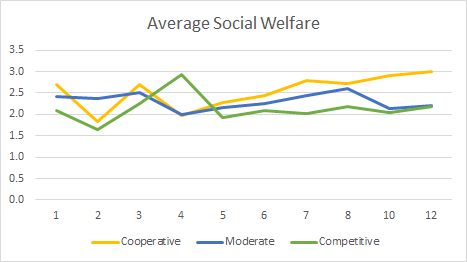
\includegraphics[width=\linewidth]{pre/180_social_welfare}
	\caption{180 Rounds per Opponent}
	\label{fig:180_social_welfare}
	\endminipage\hfill
\end{figure}

\subsection{Cooperative utilities}

Finally we take a look at the achieved utilities. Starting with cooperative in Figure \ref{fig:18_utils_domain_cooperative} and \ref{fig:180_utils_domain_cooperative}, we perform less in the long negotiation compared to the short negotiation. On average we perform equal to our opponents in the short negotiations, where we are clearly outperformed in the long run.\\

\begin{figure}[H]
	\minipage{0.49\textwidth}
	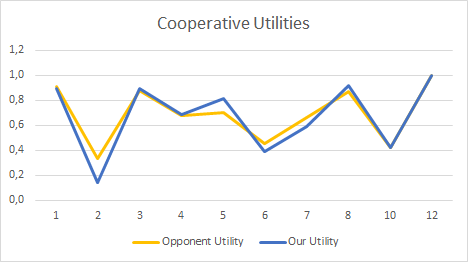
\includegraphics[width=\linewidth]{pre/18_utils_domain_cooperative}
	\caption{18 Rounds per Opponent}
	\label{fig:18_utils_domain_cooperative}
	\endminipage\hfill
	\minipage{0.49\textwidth}
	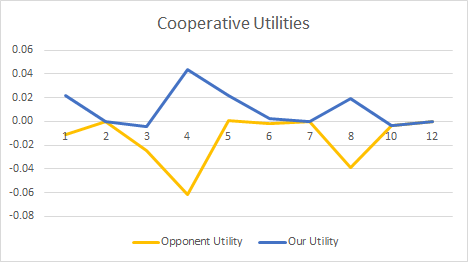
\includegraphics[width=\linewidth]{pre/180_utils_domain_cooperative}
	\caption{180 Rounds per Opponent}
	\label{fig:180_utils_domain_cooperative}
	\endminipage\hfill
\end{figure}

\subsection{Moderate utilities}

Secondly the utilities from the moderate domain, shown in Figure \ref{fig:18_utils_domain_moderate} and \ref{fig:180_utils_domain_moderate}. Again, these are mostly equal, with the exception of Opponent 5 outperforming us and Opponent 12 performing less (in the long negotiations). 

\begin{figure}[H]
	\minipage{0.49\textwidth}
	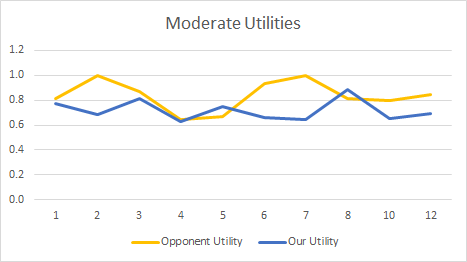
\includegraphics[width=\linewidth]{pre/18_utils_domain_moderate}
	\caption{18 Rounds per Opponent}
	\label{fig:18_utils_domain_moderate}
	\endminipage\hfill
	\minipage{0.49\textwidth}
	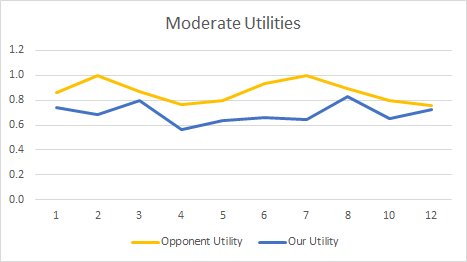
\includegraphics[width=\linewidth]{pre/180_utils_domain_moderate}
	\caption{180 Rounds per Opponent}
	\label{fig:180_utils_domain_moderate}
	\endminipage\hfill
\end{figure}

\subsection{Competitive utilities}

Without trying to sound too repetitive, looking at the competitive utilities in  Figure \ref{fig:18_utils_domain_competitive} and \ref{fig:180_utils_domain_competitive}, we see again that opponent 5 and 12 seem to have the same behavior when comparing the short and long negotiations, with our own performance being less in the long term.

\begin{figure}[H]
	\minipage{0.49\textwidth}
	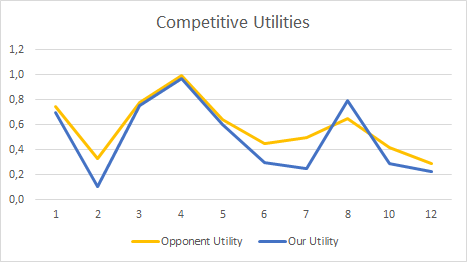
\includegraphics[width=\linewidth]{pre/18_utils_domain_competitive}
	\caption{18 Rounds per Opponent}
	\label{fig:18_utils_domain_competitive}
	\endminipage\hfill
	\minipage{0.49\textwidth}
	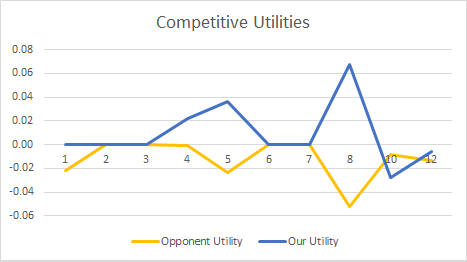
\includegraphics[width=\linewidth]{pre/180_utils_domain_competitive}
	\caption{180 Rounds per Opponent}
	\label{fig:180_utils_domain_competitive}
	\endminipage\hfill
\end{figure}